\documentclass[12pt,spanish]{article}
\usepackage[spanish]{babel}
\usepackage{graphicx}
\usepackage{color}
\usepackage{xcolor}
\usepackage{colortbl}
\usepackage{amsthm,thmtools}
\usepackage{multirow}
\usepackage{amsmath}
\usepackage{subcaption}
\usepackage{adjustbox}
\usepackage{multirow}
\usepackage[hidelinks]{hyperref}
\usepackage{caption}
\usepackage{amsthm}
\usepackage{multicol}
\usepackage[outputdir=build]{minted}
\usepackage{float}
\usepackage{amsfonts}
\usepackage{titling}
\usepackage{soul}
\usepackage{listings}
\usepackage{array}
\graphicspath{ {./img/} {../../LaTeX/img/}}
\selectlanguage{spanish}
\usepackage[utf8]{inputenc}
\usepackage{graphicx}
\usepackage[a4paper,left=3cm,right=2cm,top=2.5cm,bottom=2.5cm]{geometry}


\makeatletter
\patchcmd\thmt@mklistcmd
  {\thmt@thmname}
  {\check@optarg{\thmt@thmname}}
  {}{}
\patchcmd\thmt@mklistcmd
  {\thmt@thmname\ifx}
  {\check@optarg{\thmt@thmname }\ifx}
  {}{}
\protected\def\check@optarg#1{%
  \@ifnextchar\thmtformatoptarg\@secondoftwo{#1}%
}
\makeatother


\newtheorem{definition}{Definición}
\numberwithin{definition}{subsection}
\renewcommand{\listtheoremname}{Índice de definiciones}



\title{Fundamentos de Bases de Datos}
\setlength{\droptitle}{10em}
\author{Carlos Sánchez Páez}

\makeindex
\begin{document}


\begin{titlepage}

\newlength{\centeroffset}
\setlength{\centeroffset}{-0.5\oddsidemargin}
\addtolength{\centeroffset}{0.5\evensidemargin}
\thispagestyle{empty}

\noindent\hspace*{\centeroffset}
\begin{minipage}{\textwidth}

\centering

\includegraphics[width=0.9\textwidth]{logo_ugr.jpg}\\[1.4cm]

\textsc{ \Large Fundamentos de Bases de Datos\\[0.2cm]}
\textsc{GRADO EN INGENIERÍA INFORMÁTICA}\\[1cm]

{\Huge\bfseries Resumen del temario\\}
\end{minipage}

\vspace{1.5cm}
\noindent\hspace*{\centeroffset}
\begin{minipage}{\textwidth}
\centering

\textbf{Autor}\\ {Carlos Sánchez Páez}\\[2.5ex]

\includegraphics[width=0.3\textwidth]{etsiit_logo.png}\\[0.1cm]
\vspace{1.5cm}

\includegraphics[width=0.5\textwidth]{decsai.jpg}\\[0.1cm]
\vspace{1cm}
\textsc{Escuela Técnica Superior de Ingenierías Informática y de Telecomunicación}\\
\vspace{1cm}
\textsc{Curso 2017-2018}
\end{minipage}
\end{titlepage}
\thispagestyle{empty}
\newpage
\tableofcontents{}
\newpage
\listoffigures
\listoftheorems
\thispagestyle{empty}
\newpage

\section{Tema 1. Introducción y definiciones iniciales.}

\subsection{Concepto intuitivo de bases de datos}

Prácticamente todas las empresas necesitan aplicacioens que gestionen información a la que se accederá desde distintos puntos. Si estos datos pertenecen a las aplicaciones, hay tres problemas principales:
\begin{itemize}
	\item \textbf{Redundancia}. La información se repite en varios sitios a la vez.
	\item \textbf{Inconsistencia}. ¿Cuáles son los datos más actualizados?
	\item \textbf{No hay reutilización}. 
\end{itemize}

Si utilizamos ficheros, podemos hacer que la información sea compartida, sin embargo:
\begin{itemize}
	\item Tenemos que mantener una estructura determinada.
	\item Debemos proteger los archivos de ciertos usuarios.
	\item Debemos permitir el acceso con distintos lenguajes y sistemas operativos.
\end{itemize}

\begin{figure}[H]
\centering
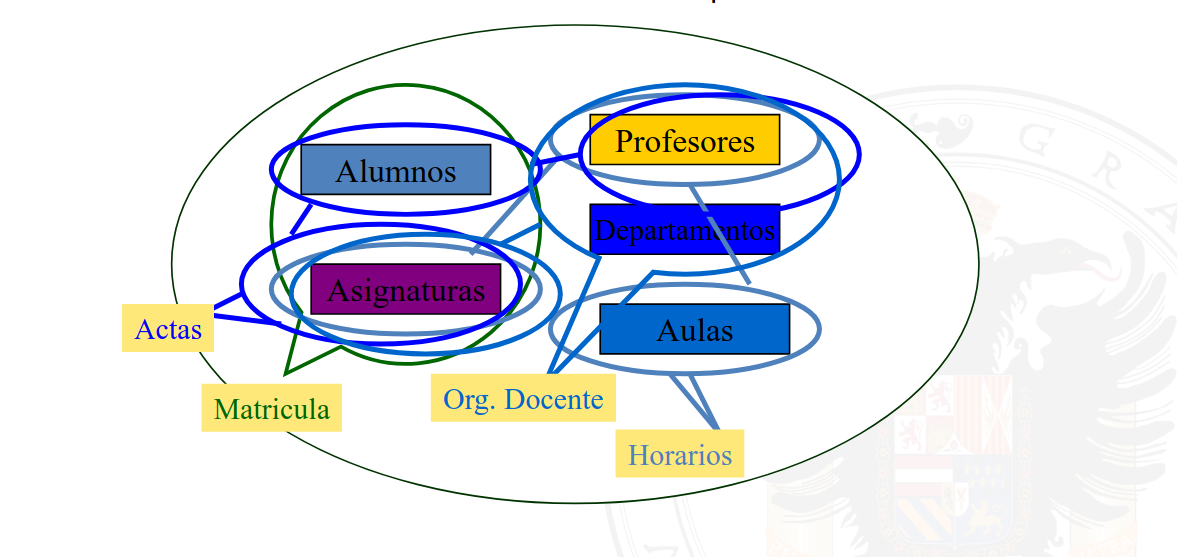
\includegraphics[scale=0.25]{redundancia_archivos.png}
\caption{Acceso a archivos desde diferentes aplicaciones.}
\end{figure}

Por tanto, la solución final es \textbf{una base de datos}.

\begin{definition}[Base de datos]
Una \emph{base de datos} es un conjunto de datos comunes a un \textit{proyecto} almacenados sin redundancia para ser útiles a distintas aplicaciones.
\end{definition}

\begin{definition}[Sistema gestor de bases de datos]
Un \emph{sistema gestor de bases de datos (SGBD)} es un conjunto de elementos software con la capacidad para definir, mantener y utilizar una base de datos.
\end{definition}

Un SGBD debe permitir:
\begin{itemize}
\item \textbf{Definir} estructuras de almacenamiento.
\item \textbf{Acceder} a los datos de forma eficiente y segura.
\item Organizar la \textbf{actualización} de los datos y el \textbf{acceso} multiusuario.
\item etc.
\end{itemize}

Resumiendo, una base de datos es un fondo común de información almacenada en una computadora para que cualquier persona o programa autorizado pueda acceder a ella, independientemente del lugar de procedencia  y el uso que haga de la misma.\\

Con un SGBD podemos gestionar datos y una estructura de datos de forma transparente (sin tener que programar un código específico):
	\begin{itemize}
		\item \textbf{Insertar} datos.
		\item \textbf{Modificar} datos existentes.
		\item \textbf{Borrar} datos existentes.
		\item \textbf{Obtener} datos previamente insertados.
	\end{itemize}
Normalmente estas operaciones se denominan CRUD (\textbf{C}reate, \textbf{R}ead, \textbf{U}pdate y \textbf{D}elete).


\subsection{Bases de datos y sistemas de gestión de bases de datos.}

Una base de datos involucra:

\begin{itemize}
	\item \textbf{Datos}
		\begin{itemize}
			\item Integrados (sin redundancia).
			\item Compartidos (útiles a varias aplicaciones).
		\end{itemize}
		\item \textbf{Hardware}
			\begin{itemize}
				\item Base de datos normal.
				\item Base de datos distribuida.
			\end{itemize}
		\item Software \textbf{DBMS} (DataBase Management System). SOn programas par describir las estructuras y gestionar la información de la base de datos.
		\item \textbf{Usuarios}
			\begin{itemize}
				\item Usuario final.
				\item Programador de aplicaciones.
				\item Administrador (DBA ó DBM).
			\end{itemize}
\end{itemize}

\begin{definition}[Dato operativo]
Un \textbf{dato operativo} es una pieza de información básica que necesita una empresa, proyecto o aplicación para su funcionamiento.
\end{definition}

Un dato operativo puede ser:
\begin{itemize}
	\item \textbf{Ítem básico}. Elementos acerca de los que se puede pedir información (sustantivos).
	\item \textbf{Atributos}. Características de los ítems básicos (adjetivos o propiedades de los ítems).
	\item \textbf{Relaciones}. Conexiones lógicas entre ítems.
\end{itemize}

Cuando se determinan y se clasifican así todos los datos operativos obtenemos el \emph{esquema lógico} de la base de datos.\\

En el día a día, usaremos el término \textbf{campo} para referirnos a la representación de un dato o atributo en la base de datos.

Ejemplos de dato operativo:

\begin{itemize}
	\item \textbf{Ítem básico}. Estudiante, asignatura, paciente, etc.
	\item \textbf{Atributos}. Nombre, apellidos, relación, etc.
	\item \textbf{Relaciones}. Estudiante \textbf{está matriculado en} asignatura, profesor \textbf{imparte} asignatura, etc.
\end{itemize}

\begin{figure}[H]
\centering
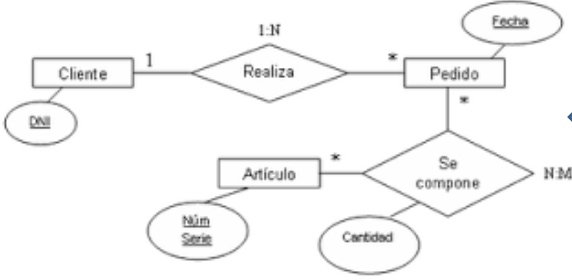
\includegraphics[scale=0.5]{ejemplo_er.png}
\caption{Ejemplo de diagrama entidad-relación.}
\end{figure}

\subsection{Concepto de independencia}

\begin{definition}[Independencia]
	Los datos se organizan independientemente de las aplicaciones que los vayan a usar de los archivos en los que vayan a almacenarse.
\end{definition}

\begin{definition}[Independencia física]
	El diseño lógico de la base de datos debe ser independiente del almacenamiento físico de los datos.
\end{definition}

Ésto permite:

\begin{itemize}
	\item Realizar cambios en la estructura física sin alterar la lógica de la aplicación (representación de campos, organización en registros, mecanismos de acceso, etc.)
	\item Liberar a las aplicaciones de la misión de gestionara aspectos relativos al almacenamiento.
\end{itemize}

\begin{definition}[Independencia lógica]
	Cada aplicación debe poder organizar lso datos según sus propios esquemas y acceder a los datos que le son necesarios y le conciernen (vistas de usuario).
\end{definition}

La independecia lógica provoca varias mejoras:
\begin{itemize}
	\item Aumento de seguridad y fiabilidad.
	\item Menos problemas para las aplicaciones.
	\item Posibilidad de cambios en los esquemas por parte de desarrolladores de aplicaciones y administradores.
\end{itemize}

El \textbf{esquema lógico general} permite organizar la información global de toda la organización para optimizar accesos, evitar redundancia, etc.\\

La \textbf{vista de usuario} permite dar permiso a los programadores de las aplicaciones para acceder a los datos que pueden ver del esquema general, ocultando los datos a los que no se debe tener acceso.\\

\subsection{Objetivos de un SGBD}

Los objetivos de un sistema de gestión de bases de datos son:

\begin{itemize}
	\item \textbf{Independencia de los datos}.
	\item \textbf{Utilización y diseño orientados al usuario}. Los datos y aplicaciones deben ser accesibles a los usuarios de la forma más amigable posible.
	\item \textbf{Centralización}. Los datos deben gestionarse de forma centralizada e independiente de las aplicaciones.
	\item \textbf{Eliminación de redundancia}. Los datos no pueden estar duplicados y se deben gestionar los accesos concurrentes.
	\item \textbf{Consistencia}. Los datos deben ser consistentes (sin fallos lógicos) y se deben implementar mecanismos para mantener la integridad.
	\item \textbf{Fiabilidad}. Los datos deben estar protegidos contra fallos, para lo que son necesarios mecanismos de mantenimiento, recuperación y realizamiento de transacciones.
	\item \textbf{Seguridad}. No todos los datos deben ser accesibles a todos los usuarios.
\end{itemize}

Hay varios tipos de usuario en una base de datos:

\begin{itemize}
	\item \textbf{Usuario final}. Debe poder acceder a los datos.
	\item \textbf{Programador de aplicaciones}. Debe eliminar problemas de diseño, depuración y mantenimiento.
	\item \textbf{Administrador}. Su cometido surge con la aparición de la base de datos.
\end{itemize}

En cuanto al sistema:

\begin{itemize}
	\item Control \textbf{centralizado}.
	\item Criterios de \textbf{uniformización}.
	\item Generación de \textbf{nuevas aplicaciones}.
	\item \textbf{Equilibrio} entre requierimientos conflictivos.
\end{itemize}

\section{Tema 2. Arquitectura de un sistema gestor de bases de datos.}

\subsection{Una arquitectura con tres niveles}
Un SGBD se organiza en niveles por varios motivos:
\begin{itemize}
	\item Los usuarios pueden acceder a los mismos datos desde distintas perspectivas, por lo que si un usuario cambia la forma de ver los datos no influye al resto.
	\item La organización global de los datos puede cambiarse sin que afecte a los usuarios.
	\item Los usuarios no tienen por qué gestionar aspectos relativos a la representación física de los datos, por lo que el administrador de la base de datos puede cambiar la representación sin que ésto influya en los usuarios.
\end{itemize}

La división se realiza en tres niveles:

\begin{definition}[NIvel interno]
Constituye la representación de la base de datos más cercana a la estructura de almacenamiento físico. Por tanto, es la capa donde se establece la forma en que se implantan las estructuras de datos que organizan los niveles superiores.
\end{definition}

\begin{definition}[Nivel conceptual]
Supone una abstracción global de la base de datos que agrupa todas las percepciones que los usuarios tienen de ella.
\end{definition}

\begin{definition}[Nivel externo]
En este nivel se definen todas las percepciones particulares de la base de datos por parte de los usuarios. Cada usuario puede tener su propia visión de la BD.
\end{definition}

\begin{figure}[H]
\centering
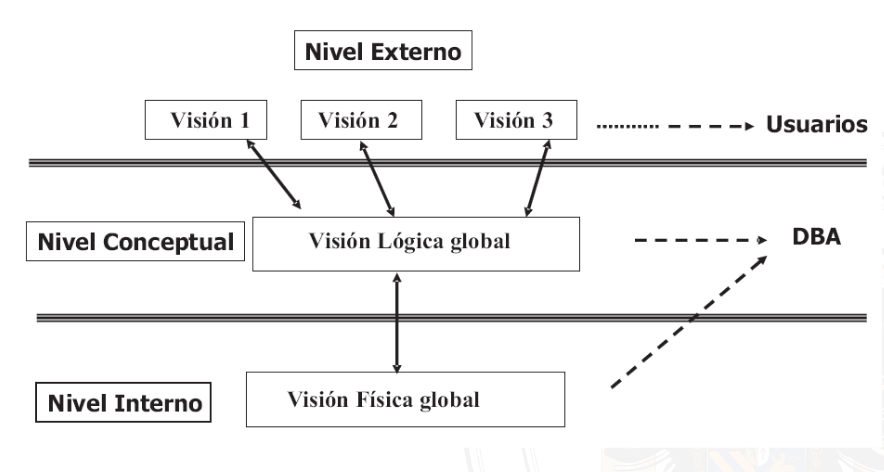
\includegraphics[scale=0.4]{tres_niveles.png}
\caption{Organización en tres niveles.}
\end{figure}

\subsubsection{Nivel externo}

Es la parte de la base de datos que es relevante para el usuario, es decir, aquellas entidades, relaciones o atributos que le son de interés. \\
Estas entidades, relaciones y atributos son representadas de la forma que le interesa al usuario (nombre completo o nombre y apellidos, etc.) y se ofrecen datos calculados a partir de ellas (edad a partir de fecha de nacimiento, etc.)

\subsubsection{Nivel conceptual}

Ofrece una visión global de los datos, así como de su estructura lógica (los datos que están almacenados y las relaciones entre ellos).\\
Éste nivel representa:
\begin{itemize}
	\item Todas las entidades, atributos y relaciones.
	\item Las restricciones que afectan a los datos.
	\item Información semántica sobre los datos.
	\item Información de seguridad e integridad.
\end{itemize}

También ofrece soporte a cada vista externa. No debe contener ningún detalle de almacenamiento.

\subsubsection{Nivel interno}

Es la representación física de la base de datos en el ordenador, es decir, la forma en la que se almacenan los datos. Busca obtener el máximo rendimiento del sistema. Representa:

\begin{itemize}
	\item Estructuras de datos.
	\item Organizaciones en ficheros.
	\item Comunicación con el sistema operativo para gestionar el uso de las unidades de almacenamiento.
	\item Compresión de datos, cifrado, etc.
\end{itemize}

Parte de las responsabilidades de este nivel son realizadas por el sistema operativo (el \emph{nivel físico}). Sin embargo, como depende de cada SGBD y de cada SO, no hay una división clara.

\begin{figure}[H]
\centering
\begin{subfigure}[b]{0.75\textwidth}
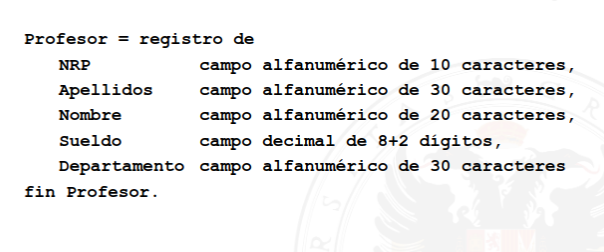
\includegraphics[width=\textwidth]{conceptual.png}
\caption{Visión conceptual.}
\end{subfigure}

	\begin{subfigure}[b]{0.4\textwidth}
		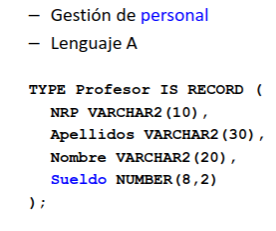
\includegraphics[width=\textwidth]{externa1.png}
		\caption{Visión externa 1.}
	\end{subfigure}
\quad
	\begin{subfigure}[b]{0.45\textwidth}
		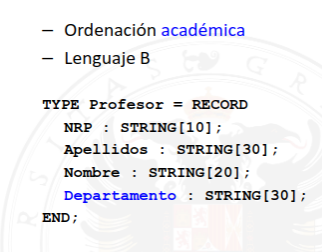
\includegraphics[width=\textwidth]{externa2.png}
		\caption{Visión externa 2.}
	\end{subfigure}

\begin{subfigure}[b]{0.75\textwidth}
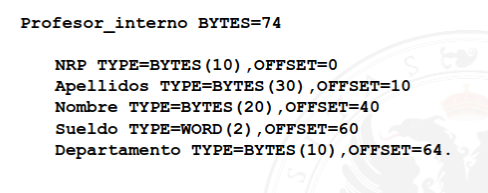
\includegraphics[width=\textwidth]{interna.png}
\caption{Visión interna.}
\end{subfigure}
\caption{Ejemplo de los tres niveles de visión.}

\end{figure}


\subsection{Correspondencias entre niveles}

\begin{definition}[Transformación o correspondencia entre niveles]
Es un conjunto de normas que establece cómo se definen los datos de un nivel en términos de otro.
\end{definition}
Es un mecanismo fundamental para establecer la independencia tanto física como lógica.

\begin{definition}[Transpormación conceptual/interna]
Define cómo se organizan las entidades lógicas del nivel conceptual en términos de registros y campos almacenados en el nivel interno.
\end{definition}

\begin{definition}[Transpormación externa/conceptual]
Describe un esquema externo en términos del esquema conceptual subyacente.
\end{definition}

Algunos SGBDs permiten la descripción de esquemas externos en términos de otros esqumas externos (transpormación externa/externa).

\begin{figure}[H]
\centering
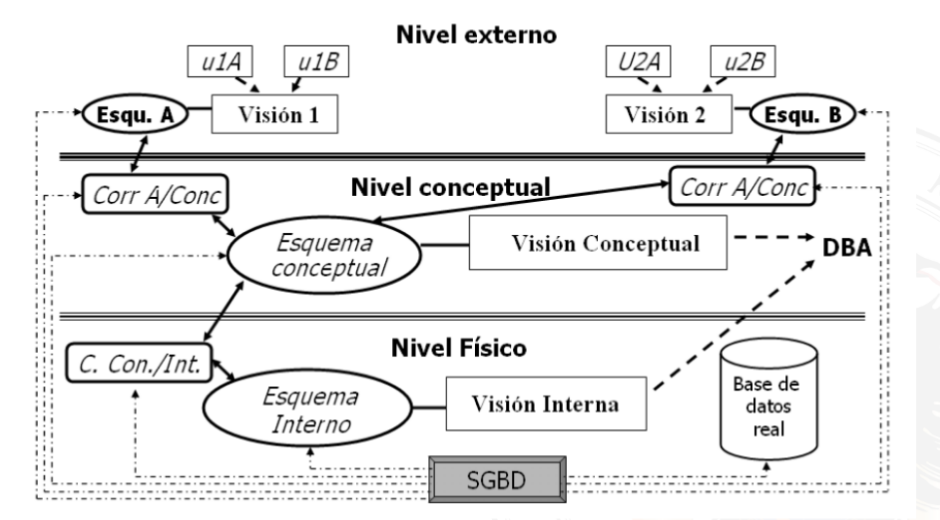
\includegraphics[scale=0.4]{correspondencia_niveles.png}
\caption{Correspondencia entre niveles.}
\end{figure}

\subsection{Lenguajes de una base de datos}

ANSI/SPARC recomienda disponer de un lenguaje específico orientado a los datos que permita definirlos, controlarlos y manipularlos.\\

\begin{definition}[DSL]
Sublenguaje de datos implementado en el propio SGBD. Consta de tres partes: DDL, DCL y DML.
\end{definition}


\begin{definition}[DDL]
\textit{(Data Definition Languaje)} o sublenguaje de definición de datos. Es el subconjunto del DSL destinado a la definición de estructuras de datos y esquemas en la base de datos.
\end{definition}

\begin{definition}[DML]
\textit{(Data Manipulation Languaje)} o sublenguaje de manipulación de datos. Es el subconjunto del DSL que permite introducir datos en los esquemas, modificarlos, eliminarlos y consultarlos. También permite consultar la estructura de los esquemas definidos en la base de datos.
\end{definition}

\begin{definition}[DCL]
\textit{(Data Control Languaje)} o sublenguaje de control de datos. Permite gestionar los requisitos de acceso a los datos y otras tareas administrativas de la base de datos.
\end{definition}

ANSI/SPARC propone disponer de un \emph{DDL}, un \emph{DML} y un \emph{DCL} para cada nivel de la arquitectura.\\

En la práctica, estos lenguajes se presentan bajo una \textbf{única implementación} en la que cada sentencia trabajará sobre uno o varios niveles. Un sistema de privilegios será el encargado de discriminar quién puede ejecutar qué y en qué nivel.\\

Como la industria ha seguido diferentes caminos, han surgido diferentes lenguajes de datos diferentes a la par que intentos por estandarizarlos (como SQL y sus estandarizaciones SQL89,SQL92, etc.).\\

Los SGBD deben tener un lenguaje anfitrión en el que están programados. Pueden ser de dos tipos:

\begin{itemize}
	\item De \textbf{propósito general}: C, C++, Java, C\#, etc.
	\item Herramientas de desarrollo \textbf{específicas}: Developer de Oracle, Oracle Application Express (Oracle APEX), Sysbase PowerBuilder, etc.
\end{itemize}

Estos lenguajes proporcionan un procesamiento avanzado de datos y la gestión de la interfaz de usuario.\\

Es necesario establecer un mecanismo para trasladar las estructuras de datos y las operaciones desde la base de datos al entorno de procesamiento de la aplicación. Surgen así dos tipos de acoplamiento:

\paragraph{Débil}
Se utilizan lenguajes de propósito general. En ellos el programador puede distinguir sentencias propias del lenguaje anfitrión y sentencias que acceden a la BD a partir de DSL.

Las principales alternativas para implementarlos son las APIs de acceso a BD (ODBC, JDCB) y el DSL inmerso en el código fuente del lenguaje anfitrión (el programador programa un código híbrido entre lenguaje anfitrión y sentencias DLS y este código pasa por un preprocesador).
\paragraph{Fuerte}

Se utilizan las herramientas de propósito especifico. Consiste en incorporar características al DSL para facilitar el desarrollo de aplicaciones.

Las principales alternativas para su implementación son PL de Oracle o la ejecución de Java sobre una máquina virtual implantada en el SGBD.

\subsection{Enfoques para la arquitectura de un SGBD}

Inicialmente, el esquema de la base de datos era centralizado:
\begin{itemize}
	\item Toda la carga de gestión y procesamiento de la información recaía en servidores centrales.
	\item El acceso se relizaba mediante terminales.
	\item En el ordenador principal se alojaban el SGBD y los programas de aplicación.
\end{itemize}

\begin{figure}[H]
\centering
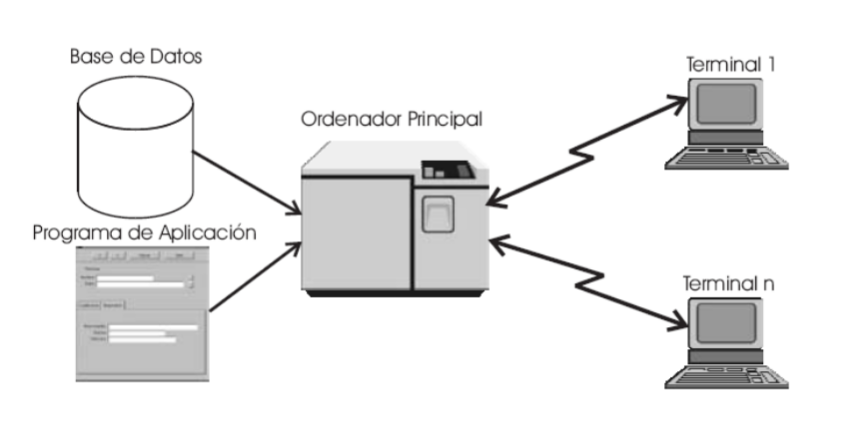
\includegraphics[scale=0.4]{arq_centralizada.png}
\caption{Arquitectura centralizada.}
\end{figure}

Esta arquitectura tenía un problema principal: el elevado coste de los ordenadores principales.\\
La solución propuesta fue desplazar la ejecución de los programas de usuario y la interacción hasta los emergentes PCs, reduciendo los costes en hardware. De esta forma, se conseguía una aproximación al modelo cliente/servidor.\\

\begin{itemize}
	\item \textbf{Servidor}. Es el servidor de la base de datos y de escucha de peticiones.
	\item \textbf{PCs conectados en red con el servidor}. Programas de aplicación y el servicio de enlace cliente que interactúa con el servicio de escucha instalado en el servidor.
\end{itemize}

El desarrollo de las redes de comunicaciones conllevó un enfoque distribuido para los servidores.

\begin{figure}[H]
\centering
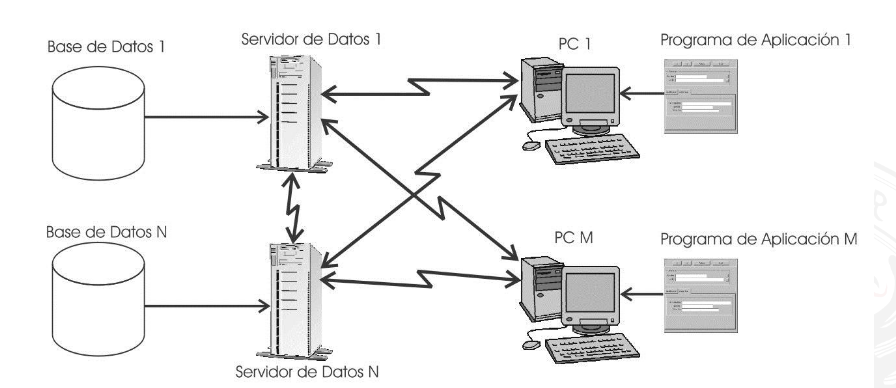
\includegraphics[scale=0.4]{arq_distribuida.png}
\caption{Arquitectura distribuida.}
\end{figure}

Sin embargo, esta arquitectura también ofrecía un gran problema: el alto coste de mantenimiento de los PCs (instalación, configuración y actualización). La solución fue separar el sistema en aplicaciones: una parte que interactúa con el usuario (\textit{interfaz de usuario}) y otra parte que se encarga de la ejecución lógica del programa.\\

Actualmente las bases de datos se estructuran en tres niveles de procesamiento:

\begin{itemize}
	\item \textbf{Nivel de servidor de datos}.
		\begin{itemize}
			\item Posiblemente distribuido.
			\item El SGBD permite organizar la información de la empresa como una BD global.
			\item Las peticiones de datos formuladas desde una sede se traducen de forma transparente a peticiones en las sedes donde se encuentran esos datos.
		\end{itemize}
		\item \textbf{Nivel de servidor de aplicaciones}. Son evoluciones de servidores web que proporcionan los programas de aplicación a clientes ligeros.
		\item \textbf{Nivel de cliente}. PCs ligeros dotados de configuraciones basadas en estándares abiertos. En muchos casos se pueden ejecutar las aplicaciones en un navegador web que soporte \textit{javascript} y \textit{html} avanzado.
\end{itemize}

\begin{figure}[H]
\centering
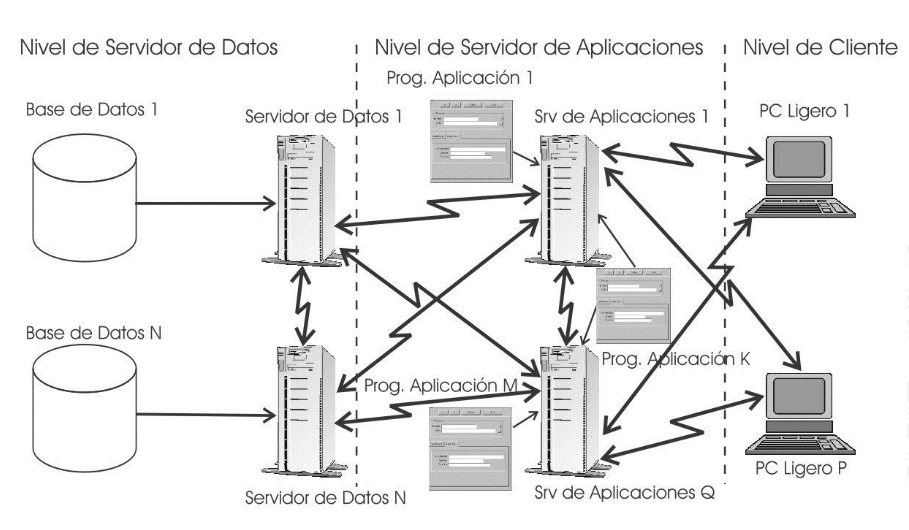
\includegraphics[scale=0.4]{arq_tres_niveles.png}
\caption{Arquitectura de tres niveles.}
\end{figure}

\paragraph{Ventajas de la arquitectura de tres niveles}

\begin{itemize}
	\item Reducción de costes en cuanto al mantenimiento de los clientes, ya que se realiza en el servidor, no en cada cliente.
	\item Mayor facilidad y flexibilidad para el usuario, ya que puede acceder casi desde cualquier puesto o dispositivo.
\end{itemize}

Su principales inconvenientes son que aumenta la complejidad a la hora de configurar y administrar servidores de aplicaciones y que es necesario desarrollar aplicaciones adaptadas a este modelo distribuido.
\newpage
\subsection{El administrador de la base de datos (DBA)}

El DBA es uina figura muy importancia en el contexto de los SGBD, ya que:
\begin{itemize}
	\item Elabora el esquema conceptual, analizando las necesidades de información de la empresa, identificando los datos operativos, elaborando el esquema lógico e implantando el esquema conceptual.
	\item Decide la estructura de almacenamiento en el nivel interno.
	\item Conecta con los usuarios mediante el análisis de requisitos, el diseño lógico, etc.
	\item Define las restricciones de integridad, como las reglas.
	\item Define e implanta la política de seguridad (gestión de usuarios y privilegios).
	\item Define e implanta la estrategia de recuperación frente a fallos (SGBDs redundantes o RAID).
	\item Optimiza el rendimiento de la BD liberando espacio no utilizado, reorganizando las operaciones para que se realicen de forma más rápida,  estableciendo prioridades. etc.
	\item Monitoriza el SGBD.
	
\end{itemize}

\newpage

\section{Tema 3. Modelos de datos.}

\begin{definition}[Modelo de datos]
Un modelo de datos es un mecanismo formal para representar y manipular información de manera general y sistemática. Debe constar de una notación para describir datos, otra para describir operaciones y otra para describir reglas de integridad.
\end{definition}

\begin{figure}[H]
\centering
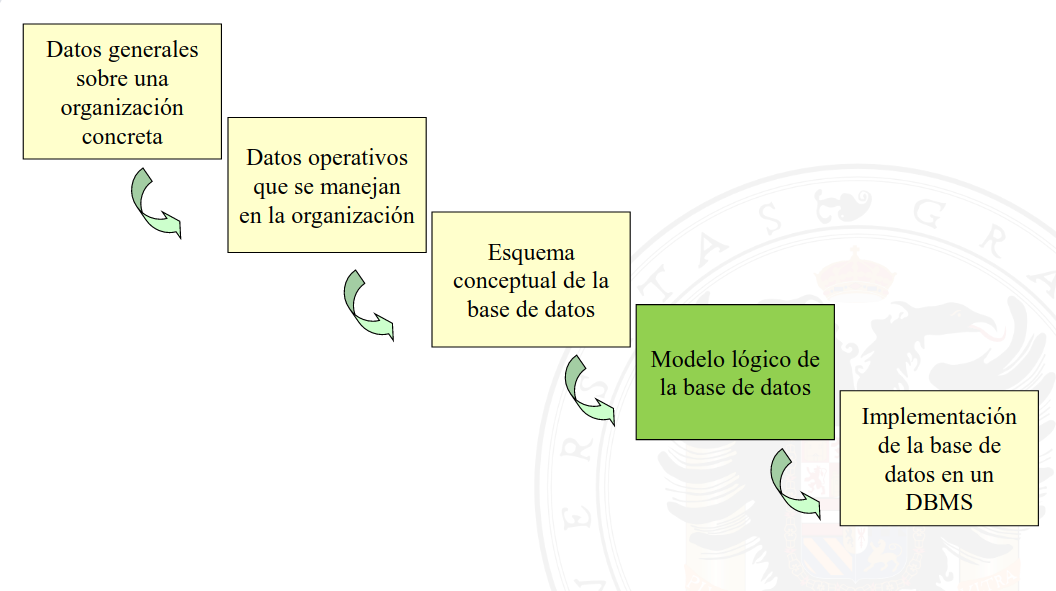
\includegraphics[scale=0.4]{pasos_bd.png}
\caption{Pasos a seguir para crear una base de datos.}
\end{figure}

Una vez llevado a cabo el proceso de análisis de datos y obtenido el esquema conceptual o \emph{lógico} de nuestra base de datos, necesitamos implantarla en un sistema a partir de un proceso de \textbf{diseño} que nos permitirá trasladar la estructura actual a un modelo de datos implementable.\\

El \textbf{modelado lógico} consiste en trasladar a un esquema lógico en función de una estructura implementable. Por último implementamos esta estructura en un sistema comercial.

Los modelos de datos son necesarios por varias razones:
\begin{itemize}
	\item Cada esquema se describe utilizando un lenguaje de definición de datos.
	\item Este lenguaje es de muy bajo nivel, muy ligado al SGBD.
	\item Hacen falta otros mecanismos de más alto nivel para poder describir los datos  de una forma no ambigua y entendible por los usuarios implicados en cada paso del proceso de implantación.
\end{itemize}


El objetivo de un modelo de datos es \textbf{describir} modelos que representen los datos y que los describan de una forma entendible y manipulable. En relación a la arquitectura ANSI/SPARC existen tres modelos: externo, conceptual e interno.\\

Los modelos de datos  pueden ser:
\begin{itemize}
	\item Basados en registros.
		\begin{itemize}
			\item  Modelo de datos \textbf{jerárquico}.
			\item  Modelo de datos \textbf{en red}.
			\item  Modelo \textbf{relacional}.
		\end{itemize}
	\item Basados en objetos.
	\item Físicos.
\end{itemize}

Los dos primeros se utilizan para los niveles externo y conceptual y el físico para el nivel interno.


\subsection{Modelo jerárquico}

Fue el primero en implementarse físicamente. En el nivel externo se utilizaban aplicaciones en \textit{Cobol} y no había interactividad (no había lenguaje de consulta).\\

Se basa en una estructura de datos básica: un árbol con registros maestro y secundarios. La base de datos es una colección de instancias de árboles.


\begin{figure}[H]
\centering
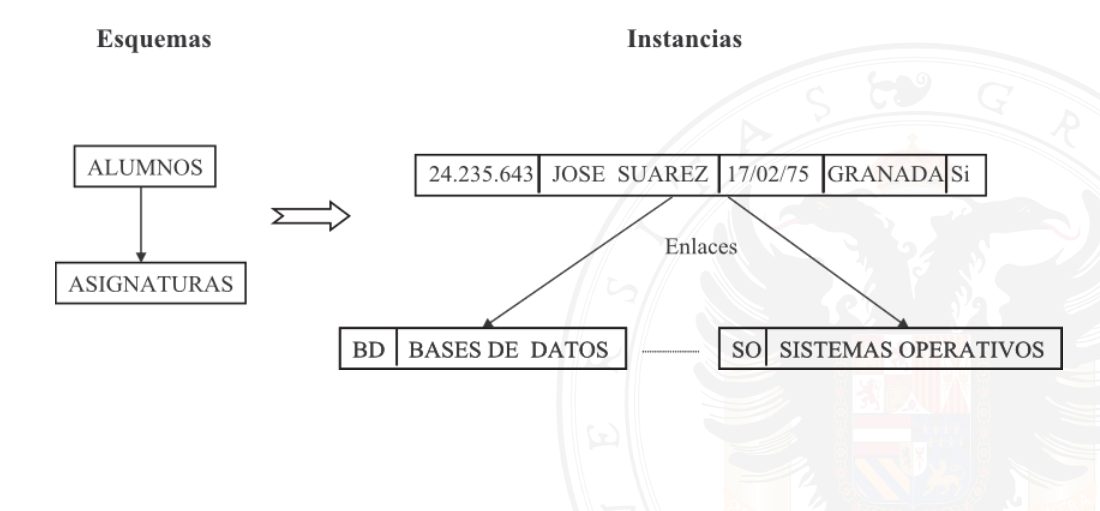
\includegraphics[scale=0.4]{modelo_jerarquico.png}
\caption{Modelo jerárquico.}
\end{figure}

Plasma de forma muy directa las relaciones muchos a uno y uno a uno. Sin embargo, tenemos que duplicar la información de las entidades involucradas en relaciones muchos a muchos.

\begin{figure}[H]
\centering
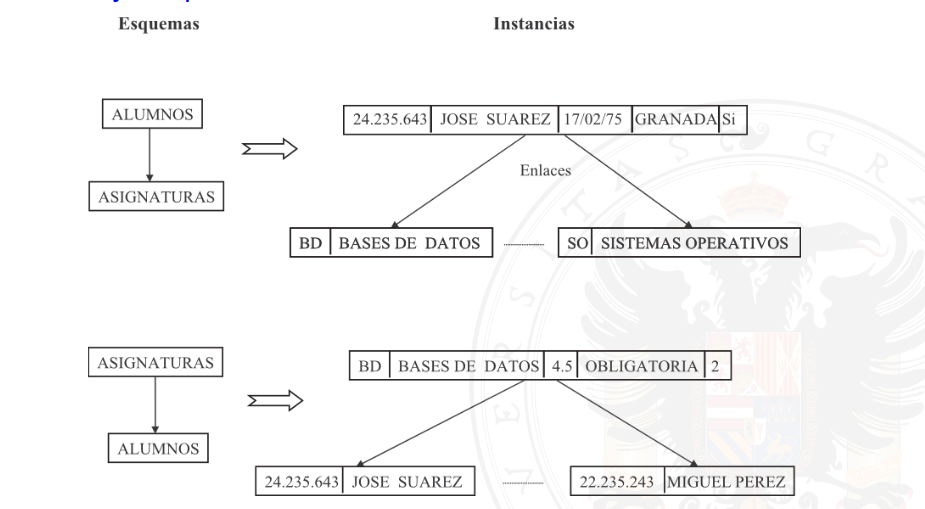
\includegraphics[scale=0.4]{jerarquico_muchos_a_muchos.png}
\caption{Relaciones muchos a muchos en el modelo jerárquico.}
\end{figure}

Sus principales inconvenientes son:

\begin{itemize}
	\item Almacenar árboles es complejo (mantenimiento de punteros y variedad de tipos de registros).
	\item El DML es difífil de usar e implementar.
	\item Dependencia existencial obligatoria de los registros secundarios con respecto a los de tipo raíz (no se puede insertar un registro secundario sin uno raíz donde \emph{engancharlo}).
	\item Redundancia al plasmar relaciones muchos a muchos.
\end{itemize}

\subsection{Modelo en red}

Su estructura de datos son grafos cuya topología depende de las conexiones entre las entidades.
\begin{itemize}
	\item Nodos $\rightarrow$ registros.
	\item Arcos $\rightarrow$ enlaces entre registros (punteros).
	\item Relaciones entre conjuntos de entidades $\rightarrow$ conectores (registros especiales). Cada ocurrencia de un conector representa una asociación distinta.
	\item Cualquier registro puede relacionarse con cualquier registro.
\end{itemize}

La base de datos se estructura como una colección de instancias de grafos.\\

La estructura es muy genérica: permite plasmar todo tipo de relaciones e implementa directamente las relaciones muchos a muchos.

\begin{figure}[H]
\centering
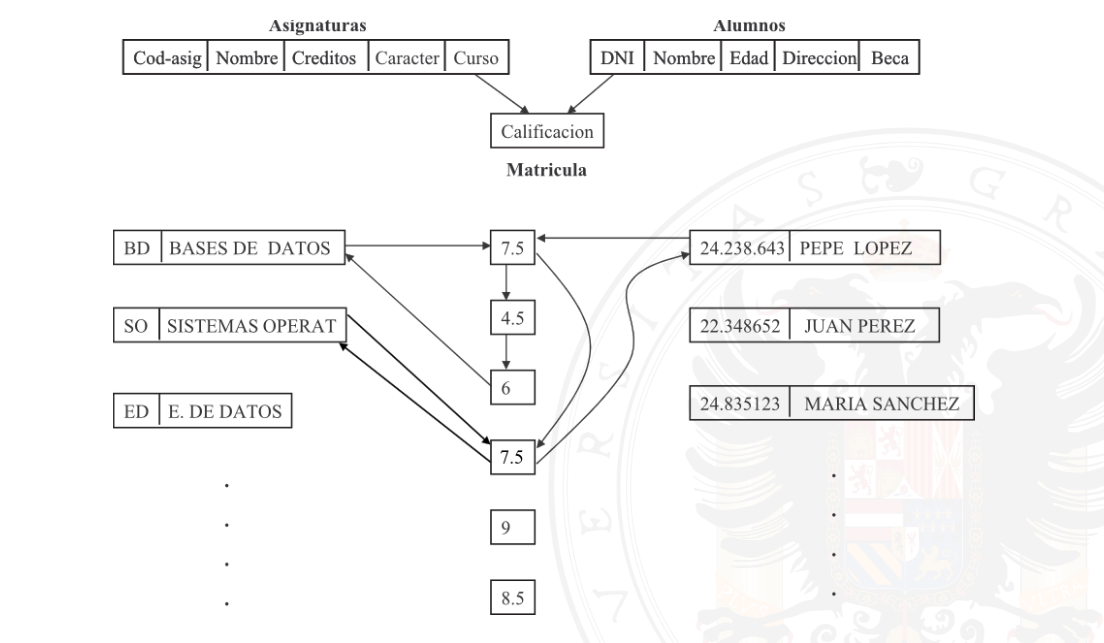
\includegraphics[scale=0.4]{modelo_red.png}
\caption{Modelo en red.}
\end{figure}

Sus principales ventajas son que la estructura es más homogénea y que permite insertar nuevas entidades de forma independiente.\\
Sin embargo, la existencia de enlaces entre registros hace que las operaciones del DDL y el DML sean complejas de implementar y utilizar.

\subsection{Modelo relacional}


Organiza y representa los datos en forma de tablas o relaciones. Una base de datos relacional es una colección de tables cada una de las cuales tiene un nombre único.

\begin{figure}[H]
\centering
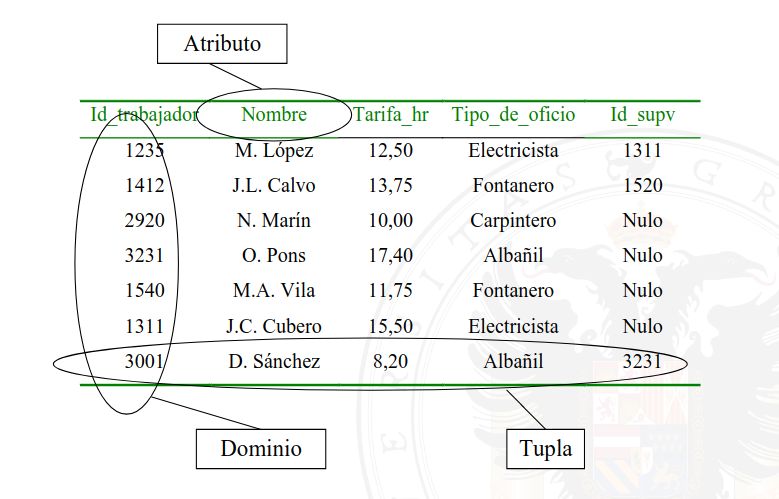
\includegraphics[scale=0.4]{modelo_relacional.png}
\caption{Modelo relacional.}
\end{figure}

\begin{definition}[Esquema de una base de datos relacional]
	Colección de esquemas de relaciones junto con restricciones de integridad.
\end{definition}

\begin{definition}[Instancia o estado de una base de datos]
	Colección de isntancias de relaciones que verifican las restricciones de integridad.
\end{definition}

\begin{definition}[Base de datos relacional]
	Instancia de una base de datos junto con su esquema.
\end{definition}

\paragraph{Claves}

\begin{definition}[Superclave]
	Cualquier conjunto de atributos que identifica unívocamente cada \emph{tupla} de una relación.
\end{definition}

\begin{definition}[Clave candidata]
	Es una superclave minimal.
\end{definition}

De entre las candidatas tenemos que elegir una como principal, denominada \textbf{clave primaria}.

\begin{figure}[H]
\centering
\begin{tabular}{|m{3cm}|m{6cm}|m{6cm}|}
\hline
 & \textbf{Relacional} & \textbf{Basado en grafos} \\
\hline
 & Un sólo elemento para la representación & Dos elementos para la representación \\
\textbf{Representación} & Conexiones lógicas & Conexiones en el modelo físico subyacente.\\
 & Representación de relaciones n:m simétrica. & Representación de relaciones n:m imposible en modelos jerárquicos, difícil en modelos de red. \\
 & Identidad por valor & Identidad por posición \\
 \hline
 & Consultas simétricas en jerarquías. & Consultas no simétricas en jerarquías. \\
\textbf{Consulta} & Obtención de la consulta como resultado global & Mecanismo de navegación por punteros.\\
 & Lenguajes declarativos & Lenguajes procedimentales \\
 \hline
\end{tabular}
\caption{Comparativa de modelos.}
\end{figure}
\newpage
\section{Tema 4. El modelo relacional.}


\subsection{La estructura de datos relacional}

El modelo relacional abarca tres ámbitos distintos de los datos:

\begin{itemize}
	\item \textbf{Las estructuras para almacenarlos}. El usuario percibe la información de la base de datos estructurada en tablas.
	\item \textbf{La integridad}. Las tablas deben satisfacer ciertas condiciones que preservan la integridad y coherencia de la información que contienen.
	\item \textbf{Consulta y manipulación}. Los operadores empleados por el modelo se aplican sobre tablas y devuelven tablas.
\end{itemize}

La tabla es la estructura lógica de un sistema relacional. A nivel físico, el sistema es libre de almacenar los datos en el formato más adecuado (archivo secuencial, indexado, etc.).
\subsection{Definiciones iniciales}

\begin{definition}[Atributo]
	Cualquier elemento de información susceptible de tomar valores. Notación: $A_i$
\end{definition}

\begin{definition}[Dominio]
	Rango de valores donde toma sus datos un atributo. Se considera finito. Notación: $D_i$
\end{definition}

\begin{definition}[Relación]
	Dados los atributos $A_i  \forall i \in \mathbb{N}$ con dominios $D_i  \forall i \in \mathbb{N}$, no necesariamente distintos, definimos relación asociada a $A_1,...,A_n$ y lo notaremos por $R(A_1,...,A_n)$ a cualquier subconjunto de $D_1 \times D_2 \times ,..., \times D_n$.
\end{definition}

\begin{definition}[Tupla]
	Cada una de las filas de una relación.
\end{definition}

\begin{definition}[Cardinalidad de una relación]
	Número de tuplas que contiene. Es variable en el tiempo.
\end{definition}


\begin{definition}[Esquema de una relación R]
	Atributos de la relación junto con su dominio, $A_1 : D_1,..., A_n : D_n$.
\end{definition}

\begin{definition}[Grado de una relación]
	Número de atributos de su esquema. Es invariable en el tiempo.
\end{definition}

\begin{definition}[Instancia de una relación]
	Conjunto de tuplas ${(x_1,x_2,...,x_n)} \subseteq D_1 \times D_2 \times ,..., \times D_n$ que componen una relación en cada momento.
\end{definition}

\begin{figure}[H]
\centering
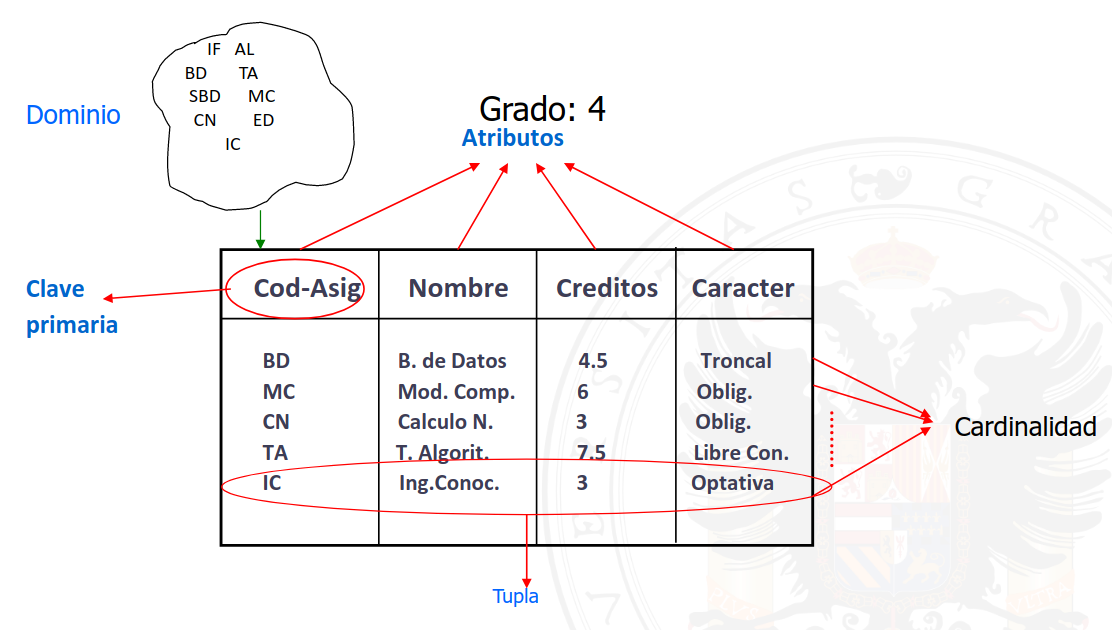
\includegraphics[scale=0.3]{elementos_relacional.png}
\caption{Ejemplo de elementos del modelo relacional.}
\end{figure}


\subsection{Propiedades de la estructura de datos relacional}

\begin{definition}[Condición de normalización]
	Todos los valores de los atributos de una relación son no atómicos (no estructurados). Cuando una relación cumple esta condición, se dice que está en \emph{primera forma normal}.
\end{definition}

La condición de normalización trae varias consecuencias:
\begin{itemize}
	\item No hay valores de tipo conjunto, registro ni tablas.
	\item No hay tuplas duplicadas.
	\item No hay orden en las filas ni en los atributos (se accede por nombre de atributo y valor).
	\item Varias instancias representan la misma relación.
\end{itemize}

Sin embargo, trae un problema: todas las representaciones son extensivas, por lo que no se puede representar información del tipo "el valor de un atributo en una tupla es igual al de otro atributo en otra tupla".

\subsection{Notación}

\begin{itemize}
	\item \textbf{Relación}. R,S,T,...
	\item \textbf{Atributos}. A,B,...
	\item \textbf{Esquema de relación}. R[$A_1,A_2,...,A_n$].
	\item \textbf{Instancia de relación R}. r.
	\item \textbf{Tuplas de una instancia}. $x_1,x_2,...,x_n \in r$.
	\item \textbf{Valor de un atributo $A_i$ en una tupla $x_j$}. $x_j[A_j]$ ó $A_{ij}$.
	\item Si no conocemos el valor de un atributo en una tupla, se le asigna un valor \textbf{nulo}.
\end{itemize}


\subsection{Restricciones o reglas de integridad}

Hay varios tipos:

\begin{itemize}
	\item \textbf{Asociada a tablas}. Ejemplos: $0 \leq edad \leq 100$, $creditos > 0$,...
	\item \textbf{Asociada a bases de datos}. Ejemplos: $imparte.NRP \in profesor.NRP$ , $cod_asig \neq nulo$.
\end{itemize}


Cuando hay más de una clave candidata en una relación, tenemos que elegir una, que será denominada \textbf{clave primaria}.

\begin{definition}[Integridad de entidad]
	No se debe permitir que una entidad sea definida en la base de datos si no tiene una información completa de sus atributos clave, es decir, la clave primaria (o una parte de ella) no puede ser nula.
\end{definition}


\begin{definition}[Clave externa]
	Conjunto de atributos de una relación que es clave en otra (o incluso en la misma) relación. Es decir, es un conjunto de atributos de una relación cuyos valores coinciden con valores de la clave primaria de las tuplas de otra relación.
\end{definition}


\begin{definition}[Integridad referencial]
	Todos los valores no nulos de una clave externa deben referenciar valores reales de la clave referenciada en la otra relación.
\end{definition}


El SGBD debe encargarse de mantener las siguientes restricciones:

\begin{enumerate}
	\item \textbf{Unicidad de clave primaria y claves candidatas}. Ante inserciones y actualizaciónes, el SGBD debe rechazar los valores que ya existan en la base de datos en las claves primarias y candidatas.
	\item\ \textbf{Restricción de integridad de identidad}. Ante inserciones y actualizaciones, se deben rechazar las modificaciones que vulneren la unicidad de la clave primaria o que le asignen algún valor nulo.
	\item \textbf{Integridad referencial}
		\begin{enumerate}
			\item En la \emph{inserción} se debe rechazar la tupla insertada si el valor de su clave externa no concuerda en la relación referenciada o si el valor es nulo y el diseño no lo permite.
			\item En la \emph{actualización}, además de verificar todo lo anterior, se debe actualizar la clave primaria de la relación referenciada.
			\item Si se \emph{borra} la clave primaria en la relación referenciada se deben borrar en cadena todas las tuplas que la referencian o poner su clave externa a valor nulo.
		\end{enumerate}
\end{enumerate}




\end{document}
